% block_diagram.tex -- detailed block diagram of cache_2way_top
% Build: tectonic block_diagram.tex   (produces block_diagram.pdf)
\documentclass[border=8pt]{standalone}
\usepackage[T1]{fontenc}
\usepackage{tikz}
\usetikzlibrary{arrows.meta, positioning, calc, fit}

\begin{document}
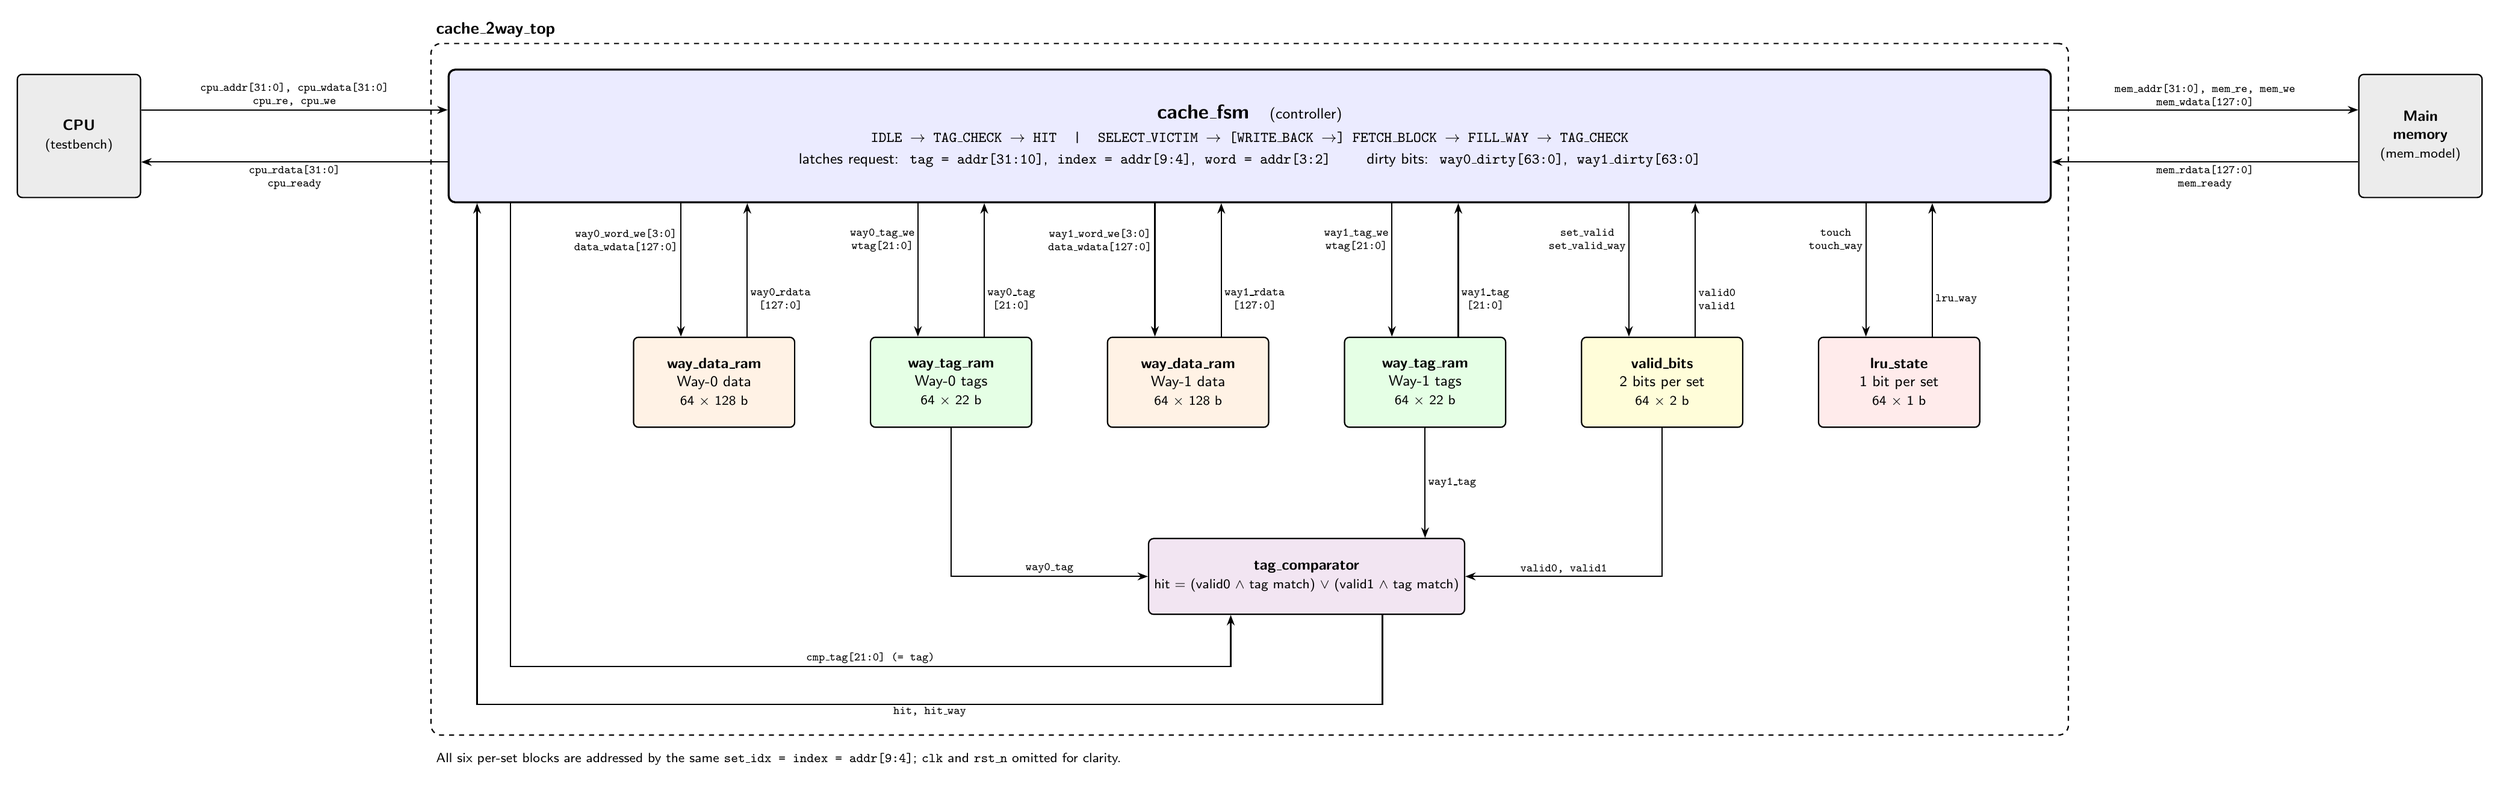
\begin{tikzpicture}[
  >={Stealth[length=2.2mm]},
  font=\sffamily\small,
  sig/.style={font=\ttfamily\scriptsize, inner sep=1.5pt, align=center},
  blk/.style={draw, thick, rounded corners=3pt, fill=#1, minimum width=3.4cm,
              minimum height=1.9cm, align=center},
  blk/.default=white,
  ext/.style={draw, thick, rounded corners=3pt, fill=gray!15, minimum width=2.6cm,
              minimum height=2.6cm, align=center},
  bus/.style={->, thick},
]

% ---------------------------------------------------------------- controller
\node[draw, very thick, rounded corners=4pt, fill=blue!8, minimum width=33.8cm,
      minimum height=2.8cm, align=center] (fsm) at (11.3,0) {%
  \textbf{\large cache\_fsm} \quad (controller)\\[3pt]
  \texttt{IDLE $\to$ TAG\_CHECK $\to$ HIT \;\;|\;\; SELECT\_VICTIM $\to$ [WRITE\_BACK $\to$] FETCH\_BLOCK $\to$ FILL\_WAY $\to$ TAG\_CHECK}\\[2pt]
  latches request:\; \texttt{tag = addr[31:10]},\; \texttt{index = addr[9:4]},\; \texttt{word = addr[3:2]}
  \qquad dirty bits:\; \texttt{way0\_dirty[63:0]},\; \texttt{way1\_dirty[63:0]}};

% ---------------------------------------------------------- per-set storage
\def\yb{-5.2}
\node[blk=orange!10] (d0)  at (0,\yb)  {\textbf{way\_data\_ram}\\Way-0 data\\\footnotesize 64 $\times$ 128 b};
\node[blk=green!10]  (t0)  at (5,\yb)  {\textbf{way\_tag\_ram}\\Way-0 tags\\\footnotesize 64 $\times$ 22 b};
\node[blk=orange!10] (d1)  at (10,\yb) {\textbf{way\_data\_ram}\\Way-1 data\\\footnotesize 64 $\times$ 128 b};
\node[blk=green!10]  (t1)  at (15,\yb) {\textbf{way\_tag\_ram}\\Way-1 tags\\\footnotesize 64 $\times$ 22 b};
\node[blk=yellow!15] (vb)  at (20,\yb) {\textbf{valid\_bits}\\2 bits per set\\\footnotesize 64 $\times$ 2 b};
\node[blk=red!8]     (lru) at (25,\yb) {\textbf{lru\_state}\\1 bit per set\\\footnotesize 64 $\times$ 1 b};

% FSM -> block (down, left of centre) and block -> FSM (up, right of centre)
\newcommand{\link}[3]{%
  \draw[bus] ($(fsm.south -| #1.north)+(-0.7,0)$) -- ($(#1.north)+(-0.7,0)$)
     node[sig, pos=0.28, left]  {#2};
  \draw[bus] ($(#1.north)+(0.7,0)$) -- ($(fsm.south -| #1.north)+(0.7,0)$)
     node[sig, pos=0.28, right] {#3};}
\link{d0}{way0\_word\_we[3:0]\\data\_wdata[127:0]}{way0\_rdata\\{[127:0]}}
\link{t0}{way0\_tag\_we\\wtag[21:0]}{way0\_tag\\{[21:0]}}
\link{d1}{way1\_word\_we[3:0]\\data\_wdata[127:0]}{way1\_rdata\\{[127:0]}}
\link{t1}{way1\_tag\_we\\wtag[21:0]}{way1\_tag\\{[21:0]}}
\link{vb}{set\_valid\\set\_valid\_way}{valid0\\valid1}
\link{lru}{touch\\touch\_way}{lru\_way}

% ---------------------------------------------------------- tag comparator
\node[blk=violet!10, minimum width=6.4cm, minimum height=1.6cm] (cmp) at (12.5,-9.3)
  {\textbf{tag\_comparator}\\\footnotesize hit = (valid0 $\wedge$ tag match) $\vee$ (valid1 $\wedge$ tag match)};

\draw[bus] (t0.south) |- node[sig, pos=0.75, above] {way0\_tag} (cmp.west);
\draw[bus] (t1.south) -- node[sig, right] {way1\_tag} (t1.south |- cmp.north);
\draw[bus] (vb.south) |- node[sig, pos=0.75, above] {valid0, valid1} (cmp.east);

% cmp_tag down to the comparator (inner lane), hit/hit_way back up (outer lane);
% both run left of the Way-0 labels and never cross.
\draw[bus] (-4.3,0 |- fsm.south) -- (-4.3,-11.2) -| node[sig, pos=0.25, above] {cmp\_tag[21:0] (= tag)}
  ($(cmp.south)+(-1.6,0)$);
\draw[bus] ($(cmp.south)+(1.6,0)$) |- node[sig, pos=0.75, below] {hit, hit\_way}
  (-5.0,-12.0) -- (-5.0,0 |- fsm.south);

% ---------------------------------------------------------- boundary + I/O
\coordinate (bottom) at (11.3,-12.4);
\node[draw, dashed, thick, rounded corners=6pt, inner sep=10pt,
      fit=(fsm)(d0)(lru)(cmp)(bottom), yshift=4pt, minimum height=14.6cm] (top) {};
\node[anchor=south west, font=\sffamily\bfseries] at (top.north west) {cache\_2way\_top};

\node[ext] (cpu) at (-13.4,0) {\textbf{CPU}\\\footnotesize (testbench)};
\node[ext] (mem) at (36.0,0) {\textbf{Main}\\\textbf{memory}\\\footnotesize (mem\_model)};

\draw[bus] ($(cpu.east)+(0,0.55)$) -- node[sig, above] {cpu\_addr[31:0], cpu\_wdata[31:0]\\cpu\_re, cpu\_we} ($(fsm.west)+(0,0.55)$);
\draw[bus] ($(fsm.west)+(0,-0.55)$) -- node[sig, below] {cpu\_rdata[31:0]\\cpu\_ready} ($(cpu.east)+(0,-0.55)$);

\draw[bus] ($(fsm.east)+(0,0.55)$) -- node[sig, above] {mem\_addr[31:0], mem\_re, mem\_we\\mem\_wdata[127:0]} ($(mem.west)+(0,0.55)$);
\draw[bus] ($(mem.west)+(0,-0.55)$) -- node[sig, below] {mem\_rdata[127:0]\\mem\_ready} ($(fsm.east)+(0,-0.55)$);

% ---------------------------------------------------------- notes
\node[anchor=north west, align=left, font=\sffamily\footnotesize] at ($(top.south west)+(0,-0.25)$)
  {All six per-set blocks are addressed by the same \texttt{set\_idx = index = addr[9:4]};
   \texttt{clk} and \texttt{rst\_n} omitted for clarity.};
\end{tikzpicture}
\end{document}
